\documentclass{article}
\usepackage{graphicx}
\usepackage{enumitem}
\usepackage{booktabs}
\usepackage{hyperref}
\usepackage[textwidth=16cm, textheight=22cm]{geometry}

%\setlength{\oddsidemargin}{11pt}% the default is 31pt so decrease by 20pt
%\setlength{\textwidth}{430pt}% the default is 390pt so increase by 40pt

\newcommand{\imgSize}{0.40\textwidth}

\begin{document}
    \pagenumbering{gobble}

    \section*{Instructions}

    This image labeling is not about gathering more training data but instead about evaluating the current model output quality against human detection. The goal is to detect ArUco markers on photonic crystal structures on tape. Due to the manufacturing process of these structures, the markers are often not entirely visible.

    \begin{figure}[h!]
        \begin{center}
          
\includegraphics[width=0.3\textwidth]{images/in-img-marker-scaled.png}
        \end{center}
        \caption{Example of the type of ArUco marker that is supposed to be detected}
        \label{fig:marker}
    \end{figure}

    \textbf{The images should be labeled as well as possible but only recognizable ArUco markers should be labeled.}

    The labeling workflow is as follows:
    \begin{enumerate}
        \item Unzip the supplied images into a folder
        \item Navigate to \href{https://www.makesense.ai}{https://www.makesense.ai}
        \item Press "Get Started" in the bottom right, drop the images as requested and press "Object Detection"
        \item Ignore the create labels dialog and press "Start project"
        \item \textbf{Select "Polygon"} in the bottom right corner
        \item Label the images (Ctrl + Scroll to Zoom, Arrows at the bottom of the page to go to the next picture)
        \item Press top left "Actions", then "Export Annotations", choose "Single file in \textbf{COCO JSON format}.", then Export.
        \item Send the resulting file to \textit{niklas.carstensen@gmx.de} or \textit{dobiko} on Discord
        \item You are Done!
    \end{enumerate}

    \newpage

    \centerline{\Large{Examples for Markers in Images}}
    \begin{table}[h!]
        \begin{center}
        \begin{tabular}{ c c }
        Unlabeled Image & Labeled Image \\ 
        \raisebox{-\totalheight}{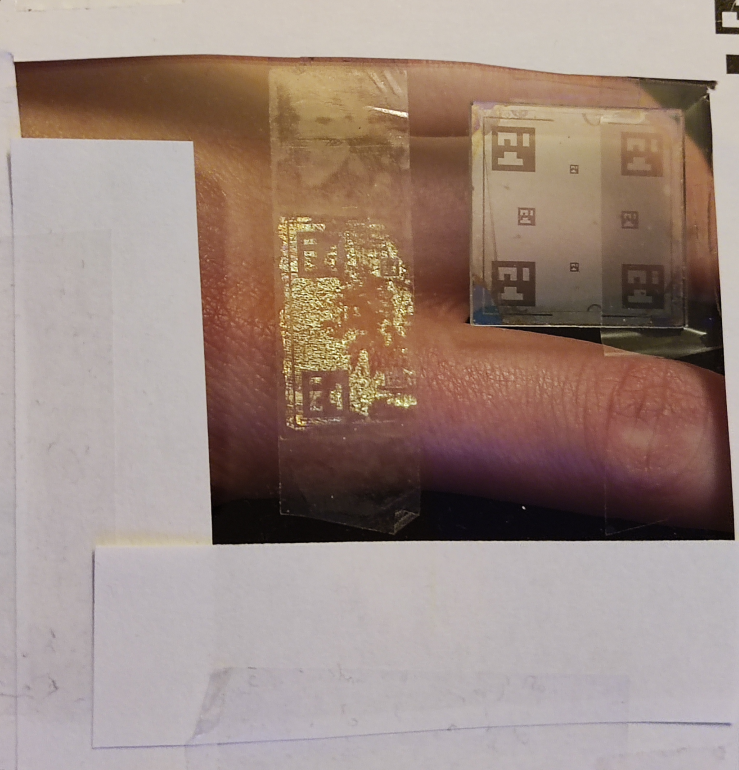
\includegraphics[width=\imgSize, height=\imgSize]{images/75_in.png}} & 
        \raisebox{-\totalheight}{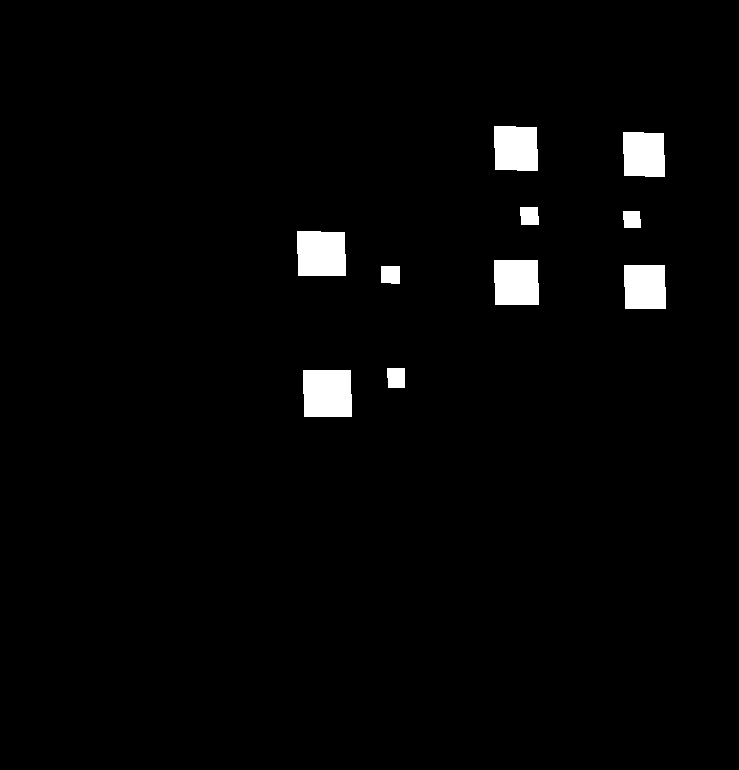
\includegraphics[width=\imgSize, height=\imgSize]{images/75_seg.png}} \\ 
        \raisebox{-\totalheight}{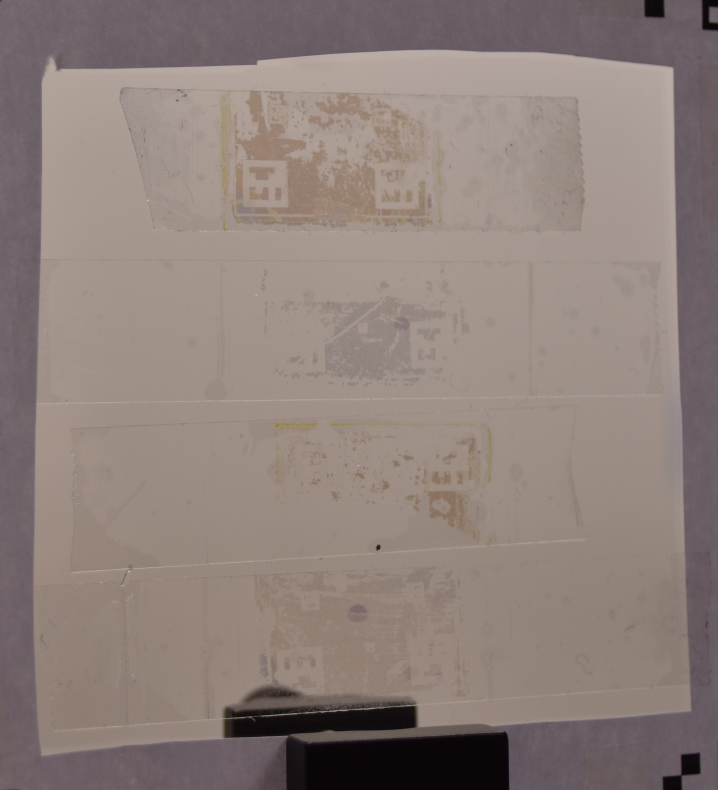
\includegraphics[width=\imgSize, height=\imgSize]{images/107_in.png}} & 
        \raisebox{-\totalheight}{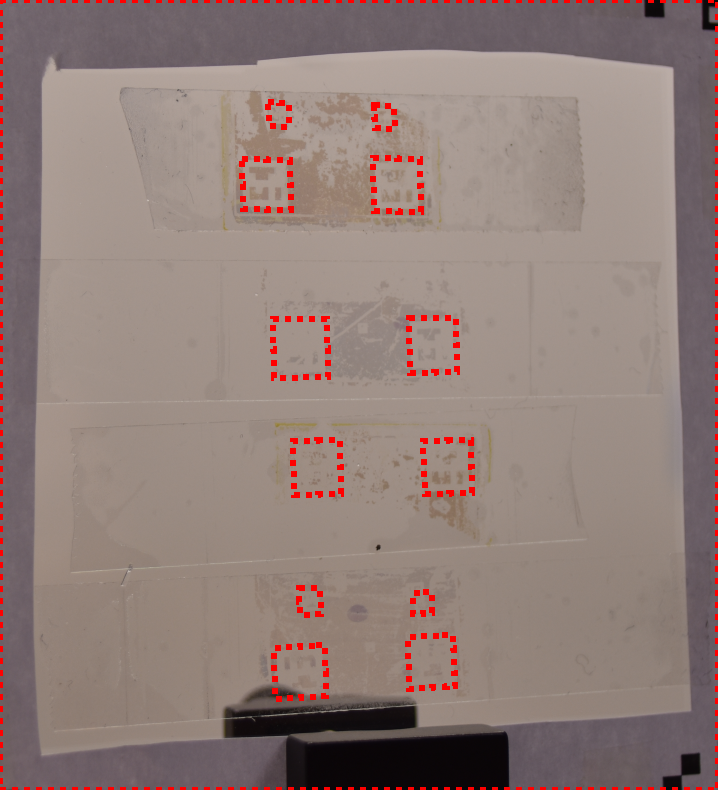
\includegraphics[width=\imgSize, height=\imgSize]{images/107_seg.png}} \\ 
        \raisebox{-\totalheight}{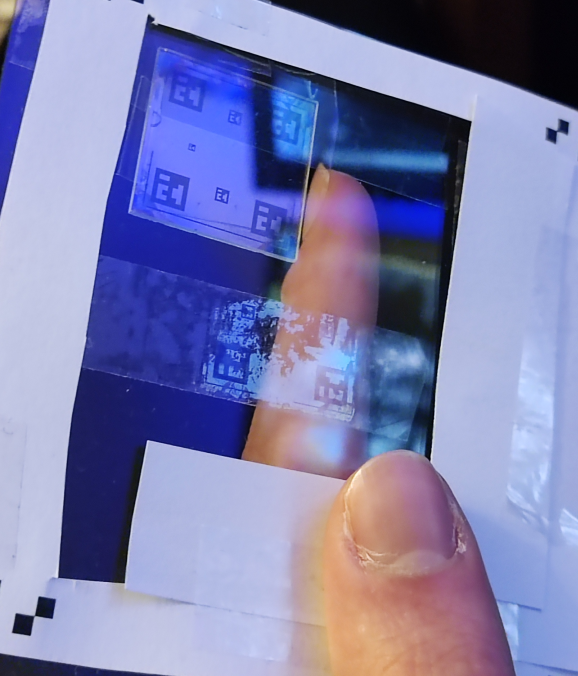
\includegraphics[width=\imgSize, height=\imgSize]{images/112_in.png}} & 
        \raisebox{-\totalheight}{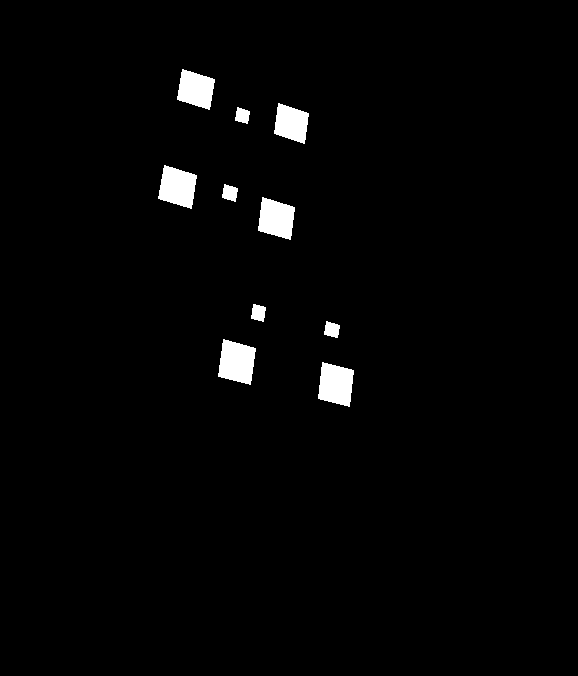
\includegraphics[width=\imgSize, height=\imgSize]{images/112_seg.png}} \\ 
        \end{tabular}
        \label{tbl:pics}
        \end{center}
    \end{table}
\end{document}
